% On utilise Beamer (pour faire des slides)
\documentclass[10pt]{beamer}

% Choix du thème
\usetheme{Madrid}

% Packages
\usepackage[utf8]{inputenc}
\usepackage{caption}
\usepackage{pgfpages} 



%%%% Page de garde du document %%%%
\title{Modeleur 3D par B-Mesh}
\author{Julien Daval \\ Omid Ghorreshi}
\institute[Ensimag 2A]{2ème année Ensimag}
\date{11 Juin 2015}
\logo{
\includegraphics[scale=0.3]{images/ensimag.jpg}}


%%%% Début du document %%%%
\begin{document}


%% Affichage de la page de garde
\begin{frame}
	\titlepage
\end{frame}


%% Sommaire
\begin{frame}
	\frametitle{Sommaire}
	\tableofcontents
\end{frame}


%% Slide d'introduction
\begin{frame}
	\frametitle{Introduction}
	\begin{block}{Principe du modeleur}
		Générer le maillage d'un objet 3D uniquement à partir de:
		\begin{itemize}
			\item Sphères;
			\item Liens entre ces sphères.
		\end{itemize}
	\end{block}
	
	\begin{center}
		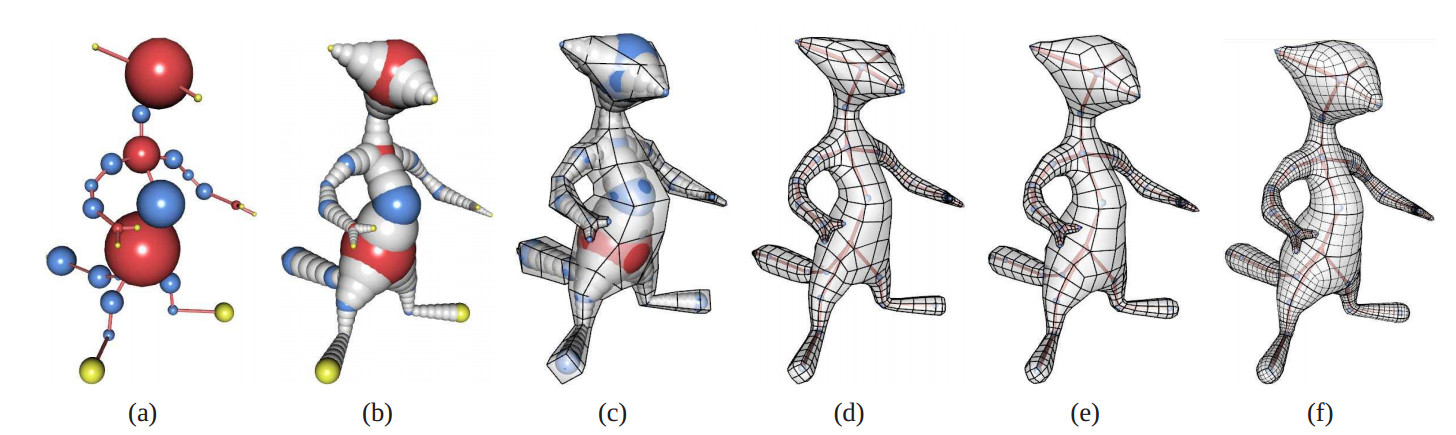
\includegraphics[scale=0.2]{images/bmesh.jpg}
	\end{center}
\end{frame}


%% Pourquoi modéliser avec des sphères ?
\section{Pourquoi modéliser avec des sphères ?}

\begin{frame}
	\frametitle{Pourquoi modéliser avec des sphères ?}
	\begin{figure}[H]
		\centering
		\leavevmode
  		\hbox{
  			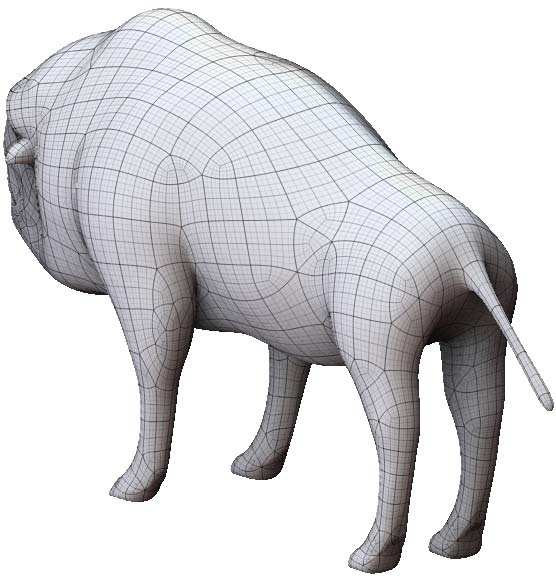
\includegraphics[scale=0.2]{images/basemesh.jpg}
  			\hspace*{0.5cm} 
     		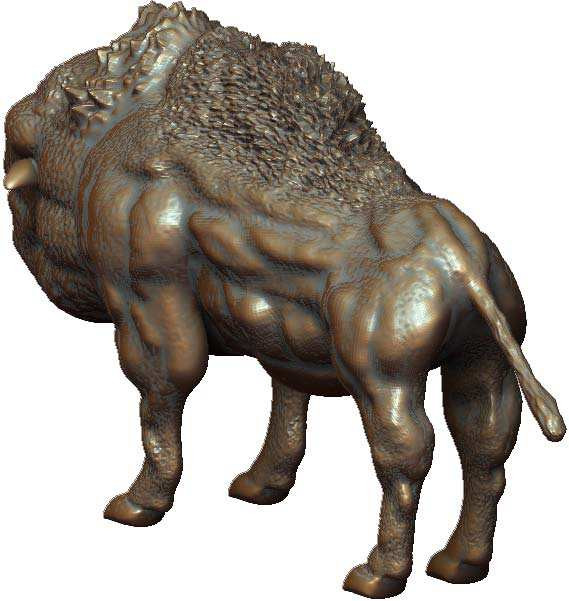
\includegraphics[scale=0.2]{images/detailedmesh.jpg}
     		\hspace*{0.5cm}  
  		}
	\end{figure}
\end{frame}


%% Interface graphique
\section{Présentation de l'outil}

% Slide 1 (screenshot)
\begin{frame}
	\frametitle{Présentation de l'outil}
	\framesubtitle{Aperçu de l'interface graphique}
	\begin{center}
		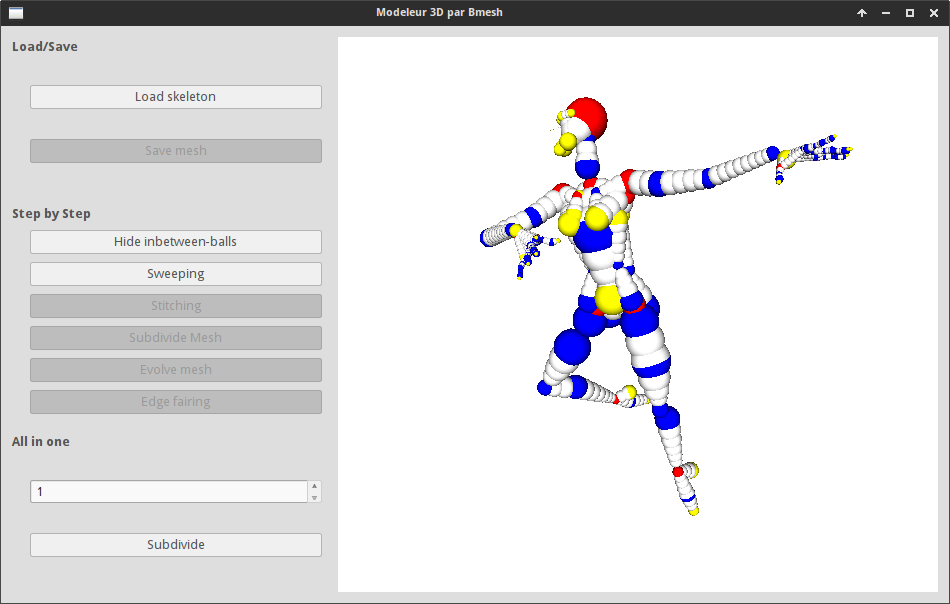
\includegraphics[scale=0.27]{images/screenshot.png}
	\end{center}
\end{frame}

% Slide 2 (description)
\begin{frame}
	\frametitle{Présentation de l'outil}
	\framesubtitle{Fonctionnalités}
	\begin{block}{Chargement / Sauvegarde}
		\begin{itemize}
			\item Chargement d'un squelette (au format .txt)
			\item Sauvegarde du maillage généré (au format .obj)
		\end{itemize}				
	\end{block}
	\begin{block}{Application de l'algorithme}
		\begin{itemize}
			\item Étape par étape...
			\item ... ou tout d'un coup (nombre d'itérations réglable)
		\end{itemize}
	\end{block}
\end{frame}



%% Algorithme
\section{Algorithme}

% Intro article
\begin{frame}
	\frametitle{À propos de l'article}
	\begin{block}{Source}
		\textit{B-Mesh: A Fast Modeling System for Base Meshes of 3D Articulated Shapes} \\
		Zhongping Ji, Ligang Liu, Yigang Wang \\
		\textit{Institute of Graphics and Image, Hangzhou Dianzi University, Chine} \\
		\textit{Department of Mathematics, Zhejiang University, Chine}
	\end{block}
\end{frame}




%%%% Fin du document %%%%
\end{document}